\documentclass[aspectratio=169]{beamer}
\usepackage[utf8]{inputenc}
\usepackage[T1]{fontenc}
\usepackage[brazil]{babel}
\usepackage{ragged2e}
\usepackage{booktabs}
\usepackage{verbatim}
\usepackage{gensymb}
\usepackage{multirow}
\usepackage{xcolor,colortbl}
\definecolor{verde}{rgb}{0,0.5,0}
\usepackage{listings}
\lstset{
  language=C++,
  basicstyle=\ttfamily\small,
  keywordstyle=\color{blue},
  stringstyle=\color{verde},
  commentstyle=\color{red},
  extendedchars=true,
  showspaces=false,
  showstringspaces=false,
%  numbers=left,
%  numberstyle=\tiny,
  breaklines=true,
  backgroundcolor=\color{green!10},
  breakautoindent=true,
  captionpos=b,
  xleftmargin=0pt
}
\newcommand\setItemnumber[1]{\setcounter{enumi}{\numexpr#1-1\relax}}

\usetheme{AnnArbor}
\usecolortheme{orchid}
\usefonttheme[onlymath]{serif}

\AtBeginSection[]{
  \begin{frame}
  \vfill
  \centering
  \begin{beamercolorbox}[sep=8pt,center,shadow=true,rounded=true]{title}
    \usebeamerfont{title}\insertsectionhead\par%
  \end{beamercolorbox}
  \vfill
  \end{frame}
}

\title[\sc{Estruturas Encadeadas}]{Estruturas Encadeadas}
\author[Roland Teodorowitsch]{Roland Teodorowitsch}
%\institute[poo - EC - PUCRS]{Laboratório de Programação II - Curso de Engenharia de Computação - PUCRS}
\institute[POO - EC - PUCRS]{Programação Orientada a Objetos - ECo - Curso de Engenharia de Computação - PUCRS}
\date{20 de outubro de 2022}

\begin{document}
\justifying

%-------------------------------------------------------
\begin{frame}
	\titlepage
\end{frame}

%=======================================================
\section{Estruturas Encadeadas}

%-------------------------------------------------------
\begin{frame}\frametitle{Estruturas Encadeadas}
\begin{itemize}
	\item Costumam ser implementadas usando alocação dinâmica, que é feita durante a execução (aumenta e diminui em tempo de execução)
	\item Os nodos são ligados entre si para indicar a relação de ordem existente entre os itens
\begin{figure}[h]
	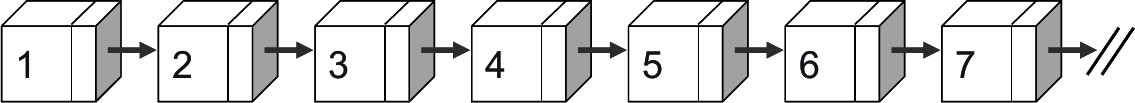
\includegraphics[height=0.12\paperheight]{pucrs-ec-poo-unidade_12-estruturas_encadeadas-laminas-estrutura_encadeada_01.png}
\end{figure}
	\item São úteis quando:
	\begin{itemize}
		\item Não é possível prever o número de entradas de dados em tempo de compilação
		\item A operação que tiver de ser feita sobre essas entradas adequar-se melhor a uma estrutura encadeada
	\end{itemize}
\end{itemize}
\end{frame}

%-------------------------------------------------------
\begin{frame}\frametitle{Estruturas Encadeadas}
\begin{itemize}
	\item Consistem de um determinado número de nodos, cada um com uma referência para o próximo nodo
	\item Duas representações usuais são:
	\begin{itemize}
		\item Encadeamento simples
\begin{figure}[h]
	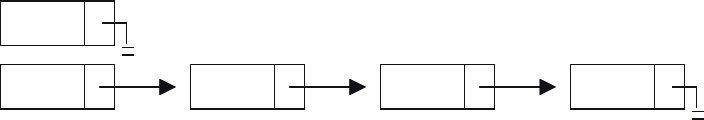
\includegraphics[height=0.14\paperheight]{pucrs-ec-poo-unidade_12-estruturas_encadeadas-laminas-estrutura_encadeada_02.png}
\end{figure}
		\item Encadeamento duplo
\begin{figure}[h]
	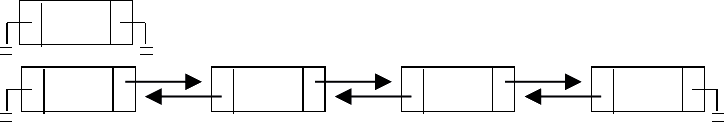
\includegraphics[height=0.15\paperheight]{pucrs-ec-poo-unidade_12-estruturas_encadeadas-laminas-estrutura_encadeada_03.png}
\end{figure}
	\end{itemize}
\end{itemize}
\end{frame}

%-------------------------------------------------------
\begin{frame}\frametitle{Estruturas Encadeadas}
\begin{itemize}
	\item Eventualmente um nodo pode armazenar mais de uma referência para outros nodos
	\item Dessa forma é possível criar estruturas de diferentes formatos
	\item Exemplo:
\begin{figure}[h]
	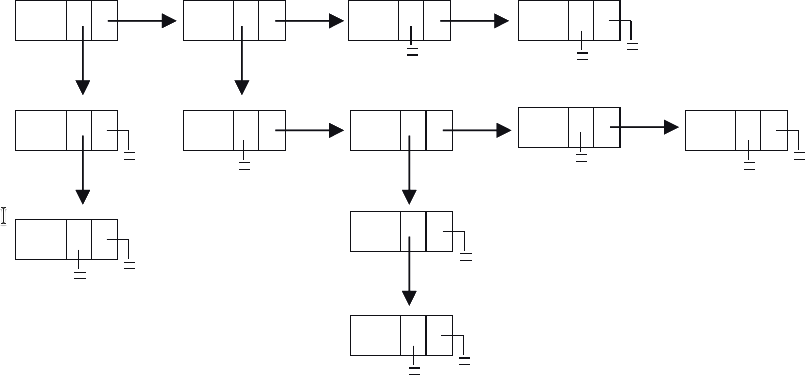
\includegraphics[height=0.5\paperheight]{pucrs-ec-poo-unidade_12-estruturas_encadeadas-laminas-estrutura_encadeada_04.png}
\end{figure}
\end{itemize}
\end{frame}

%-------------------------------------------------------
\begin{frame}\frametitle{Nodos}
\begin{itemize}
	\item Nodos são conectados (encadeados) por \emph{links}
	\item Normalmente estes nodos têm dois atributos:
	\begin{itemize}
		\item \textbf{\emph{element}} representando o elemento armazenado no nodo
		\item \textbf{\emph{next}} representando o endereço do próximo nodo no encadeamento da lista (contém referência para um objeto da mesma classe)
	\end{itemize}
\begin{figure}[h]
	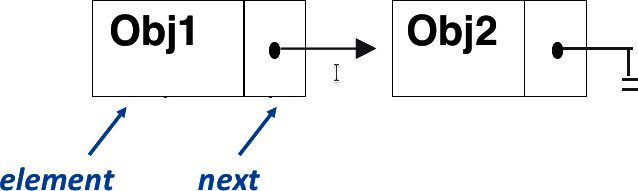
\includegraphics[height=0.2\paperheight]{pucrs-ec-poo-unidade_12-estruturas_encadeadas-laminas-estrutura_encadeada_05.png}
\end{figure}
\end{itemize}
\end{frame}

%-------------------------------------------------------
\begin{frame}\frametitle{Nodos}
\begin{itemize}
	\item Nodos podem ter mais do que dois atributos
	\item Exemplo: nodo com cinco atributos (armazena 3 elementos e possui 2 \emph{links})
\begin{figure}[h]
	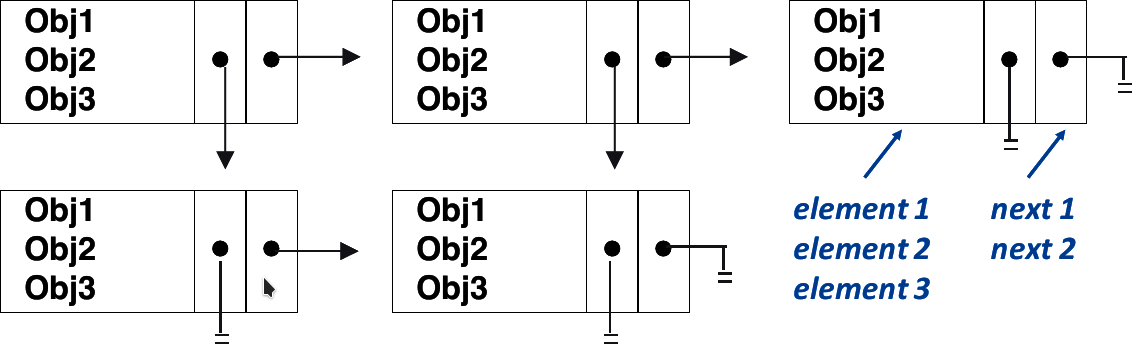
\includegraphics[height=0.3\paperheight]{pucrs-ec-poo-unidade_12-estruturas_encadeadas-laminas-estrutura_encadeada_06.png}
\end{figure}
\end{itemize}
\end{frame}

%-------------------------------------------------------
\begin{frame}\frametitle{Implementação de um Nodo}
\begin{itemize}
	\item Existem diversas opções de implementação
	\item \textbf{Classes internas privadas} são uma opção interessante
	\item Por exemplo, cria-se uma classe interna na classe que implementa uma lista encadeada
	\item Pode-se manter os atributos do nodo público sem expor sua implementação para além da implementação da própria lista encadeada
	\item Quem utiliza a lista não precisa saber que um nodo existe
\end{itemize}
\end{frame}

%-------------------------------------------------------
\begin{frame}\frametitle{Implementação de um Nodo}
\begin{itemize}
	\item \textbf{Classes internas} são classes declaradas dentro de outras classes
	\item Objetos da classe interna têm um relacionamento especial com o objeto da classe externa que o cria:
	\begin{itemize}
		\item É permitido ao objeto da classe interna acessar diretamente todos os atributos e os métodos do objeto da classe externa, não importando se são publicos ou privados
	\end{itemize}
\end{itemize}
\end{frame}

%-------------------------------------------------------
\begin{frame}[fragile]\frametitle{Implementação de um Nodo}
\begin{itemize}
	\item Exemplo: código de uma classe interna Nodo com elementos inteiros
\begin{lstlisting}[language=C++,basicstyle=\ttfamily\scriptsize]
class ListaSimplesmenteEncadeada {  // Classe externa

  private:

    class Nodo {  // Classe interna
      public:
        int elemento;
	Nodo *prox;
	Nodo(int e){
           elemento = e;
           prox = nullptr;
        }
    };

    // (...)
\end{lstlisting}
\end{itemize}
\end{frame}

%-------------------------------------------------------
\begin{frame}\frametitle{Armazenamento em Estruturas de Dados Encadeadas}
\begin{itemize}
	\item Para armazenar dados em estruturas encadeadas basta ir encadeando nodos na estrutura à medida que é necessário armazenar novas informações
	\item É fundamental armazenar uma referência para o início da estrutura encadeada de maneira a não ``perder'' os dados
	\begin{itemize}
		\item Acesso direto ao primeiro elemento (\emph{head} ou \emph{prim}) é obrigatório
		\item Acesso direto ao último elemento (\emph{tail} ou \emph{ult}) é desejável
	\end{itemize}
\begin{figure}[h]
	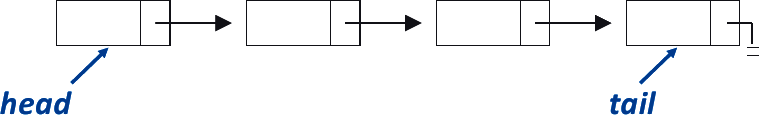
\includegraphics[height=0.15\paperheight]{pucrs-ec-poo-unidade_12-estruturas_encadeadas-laminas-estrutura_encadeada_07.png}
\end{figure}
	\item Nodos que se encontram ``nas pontas'' da estrutura podem armazenar uma referência nula (\texttt{nullptr} em C++). Desta maneira são facilmente identificados
\end{itemize}
\end{frame}

%=======================================================
\section{Lista de Exercícios}

%-------------------------------------------------------
\begin{frame}[fragile]\frametitle{Lista de Exercícios}
\begin{enumerate}
	\setItemnumber{1}
{\small
	\item Implemente uma classe \emph{ListaLinkSinal} que armazena números inteiros. Os nodos desta lista, além do dado e da referência para o próximo nodo, armazenam também uma referência para o próximo valor positivo e para o próximo valor negativo da lista (conforme a figura a seguir). Esta lista deve ter: um método \emph{add} que acrescenta elementos no final da lista; um método \emph{soPositivos} que retorna uma cadeia de caracteres com todos os valores positivos armazenados na lista; e um método \emph{soNegativos} que retorna uma cadeia de caracteres com todos os valores negativos armazenados na lista. Escreva um exemplo de uso que utilize os métodos criados.
\begin{figure}[h]
	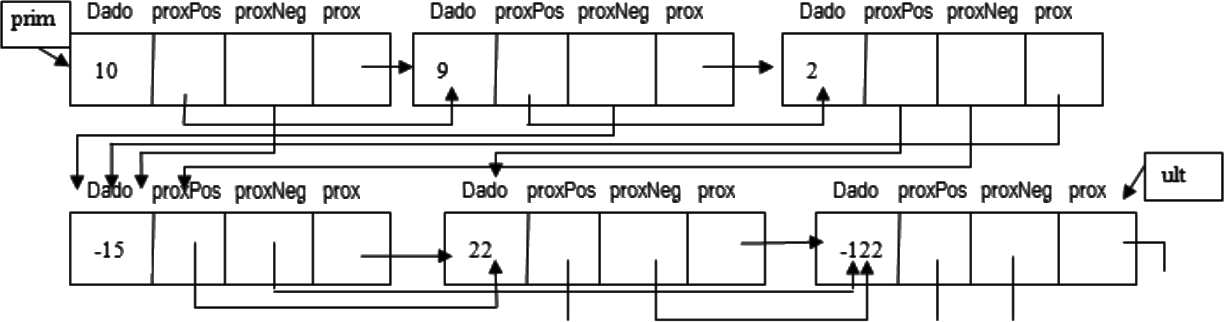
\includegraphics[height=0.35\paperheight]{pucrs-ec-poo-unidade_12-estruturas_encadeadas-laminas-estrutura_encadeada_08.png}
\end{figure}
}
\end{enumerate}
\end{frame}

%-------------------------------------------------------
\begin{frame}\frametitle{Lista de Exercícios}
\begin{enumerate}
	\setItemnumber{2}
	\item Dada a classe \emph{Pessoa}, que se encontra no Material de Apoio. Implemente a classe \emph{ListaEncadeada} que define uma lista encadeada com os métodos descritos abaixo.
	\begin{enumerate}[a)]\scriptsize{
		\item \texttt{bool estaVazia()}\\
		Informa se a lista está vazia (devolve \texttt{true}) ou não (devolve \texttt{false}).
		\item \texttt{void inserePessoaNoInicio(string nome, string endereco)}\\
		Crie um método que coloque um elemento no início da lista.
		\item \texttt{void inserePessoaNoFinal(string nome, string endereco)}\\
		Crie um método que coloque um elemento no final da lista.
		\item \texttt{Pessoa *retornaUltimo()}\\
		Retorna um apontador para o último elemento da lista. Caso a lista esteja vazia, o método deve devolver \texttt{nullptr}.
		\item \texttt{Pessoa *buscaPessoa(string nome)}\\
		Crie um método que devolva um ponteiro para um certo elemento da lista. Como parâmetro este método deve receber o nome de uma pessoa a ser buscada na lista. Caso o nome não exista na lista, o método deve devolver \texttt{nullptr}.
	}\end{enumerate}
\end{enumerate}
\end{frame}

%-------------------------------------------------------
\begin{frame}\frametitle{Lista de Exercícios}
\begin{enumerate}
	\setItemnumber{2}
	\item (Continuação)
	\begin{enumerate}[a)]\addtocounter{enumii}{5}\scriptsize{
		\item \texttt{Pessoa *buscaAnterior(string nome)}\\
		Crie um método que devolva um ponteiro para o nodo da lista que encontra-se ANTES do nodo que contém um certo elemento da lista. Como parâmetro este método deve receber o nome de uma pessoa a ser buscada na lista. Caso o nome não exista na lista ou caso o nome fornecido seja o primeiro da lista, o método deve devolver \texttt{nullptr}.
		\item \texttt{Pessoa *retira(string nome, string endereco)}\\
		Crie um método que retire um elemento da lista. Como parâmetro este método deve
receber o nome de uma pessoa a ser buscada na lista. Caso o nome não exista na lista, o
método deve devolver \texttt{nullptr}. Lembre-se de fazer um teste específico para remover o primeiro elemento da lista. O método NÃO deve ``deletar'' o nodo da memória. Dica: use o método \texttt{buscaAnterior}.
		\item \texttt{Pessoa *retiraDoInicio()}\\
		Crie um método que remova um primeiro elemento da lista. O método deve retornar um
apontador para o elemento retirado da lista. O método NÃO deve ``deletar'' o nodo da memória. Caso a lista esteja vazia, o método deve devolver \texttt{nullptr}.
	}\end{enumerate}
\end{enumerate}
\end{frame}

%-------------------------------------------------------
\begin{frame}\frametitle{Lista de Exercícios}
\begin{enumerate}
	\setItemnumber{2}
	\item (Continuação)
	\begin{enumerate}[a)]\addtocounter{enumii}{8}\scriptsize{
		\item \texttt{Pessoa *retiraDoFinal()}\\
		Crie um método que remova o último elemento da lista. O método deve retornar um apontador para o elemento retirado da lista. O método NÃO deve ``deletar'' o nodo da memória. Caso a lista esteja vazia, o método deve devolver \texttt{nullptr}.
		\item \texttt{int remove(string nome, string endereco)}\\
		Crie um método que remova um elemento da lista. O método deve ``deletar'' o nodo da memória. Dica: use o método \texttt{retira}	.
		\item \texttt{void inserePessoaEmOrdem(string nome, string endereco)}\\
		Crie um método que coloque um elemento na lista, de forma que os elementos fiquem
sempre em ordem crescente do nome da pessoa. Dica: Modifique o método de busca de
forma que ele devolva um apontador para o primeiro nodo da lista no qual o atributo
'nome' seja ``maior'' que no nome a ser inserido na lista.
	}\end{enumerate}
\end{enumerate}
\end{frame}

%=======================================================
\section{Créditos}

%-------------------------------------------------------
\begin{frame}\frametitle{Créditos}
\begin{itemize}
	\item Estas lâminas contêm trechos de materiais disponibilizados pelos professores Rafael Garibotti, Bernardo Copstein e Márcio Sarroglia Pinho (exercício 2).
\end{itemize}
\end{frame}

%-------------------------------------------------------
\end{document}

